\cotefile{75}
\scanpage{2}
% margin note written sideways in the scan, parallel to the title
\margin{(24\unsure{.} p)}
$C_{4}$\qquad DEA

\unsure{Géométries|Géometries} Combinatoires
% archive sheet number: 1

\scanpage{3}
\uline{Rappels de théorie des groupes} \uline{et sur espaces homogènes}

Groupe (loi comp. assoc. unitaire avec inverses)

hom de groupes (on a néc $f(e)=e$, $f(x^{-1})=f(x)^{-1}$)

opération d'un groupe $G$ sur un ens (ens. à groupe d'opérateurs)

opération transitive ($\forall x\mathord{.}y\in E,\ \exists g\in G,\ y=gx$) -- espace homogène

On exige \deleted{que}\inserted{de plus} $E\ne\varnothing$)
\[
\bigl(\text{couples }(E,x),\ E\ \text{esp. hom.},\ x\in E\bigr)
\Longleftrightarrow
\begin{aligned}&\text{donnée d'un ss-grpe}\\&H\ \text{de }G\end{aligned}
\]

c'est en fait une ``équivalence de catégories''

% slanted
\margin{classes d'iso. d'esp. hom. ss $G$ $\simeq$ classes de conjugaison de ss-grpes}
{\small
\diagram{\begin{tikzcd}[ampersand replacement=\&,row sep=0.6em,column sep=0.8em]
(E,x) \arrow[dd,"f"] \& \& \& {}\\
{} \& (f(x)=x') \& \Longleftrightarrow \& H\subset H'\\
(E',x') \& {\begin{aligned}&\text{\uline{NB} }f\ \text{(comm. à }G\text{) connu,}\\&\text{quand on \unsure{connait|connaît}}\\& f(x),\ \text{\uline{si} }G\ \text{trans. sur }E\end{aligned}} \& \& {}
\end{tikzcd}}}
{\small
\[
E\sim E'\quad\text{sss}\quad H,H'\ \text{conjugués}\quad\big/\quad
\exists E\to E'\quad\text{sss}\quad
\begin{aligned}&H\ \text{conjugué à un}\\[-2pt]&\text{ss-grpe de }H'\end{aligned}
\]}

\uline{Torseur sous $G$} :
{\small
\diagram{\begin{tikzcd}[ampersand replacement=\&,row sep=1.25em,column sep=1.5em]
{\left\{\begin{aligned}&\forall x,y\in E,\quad\exists 1\ g\in G,\quad gx=y\\& E\ne\varnothing\end{aligned}\right\}}
\arrow[r,Leftrightarrow] \arrow[d,Leftrightarrow] \&
{\left\{\begin{aligned}&E\ \text{\unsure{espace|esp.} hom.,}\\&\text{stabilisateur}\\&\text{\unsure{de|des} pts réd.}\\&\text{à }\{e\}\end{aligned}\right\}}\\
{\left\{E\simeq G_{s}\right\}} \&
\end{tikzcd}}}

\deleted{\unsure{Les|Le}}

Les torseurs sous $G$ sont isomorphes (non canoniquement)

Les torseurs sous $G$ sont les ``plus gros'' espaces homogènes ss $G$.

le groupe des autom. d'un torseur $P$ sous $G$ est $\sim G$ (non canonique) : le choix de $x\in P$ définit un iso. $G\overset{u_x}{\simeq}\operatorname{Aut}_{G}P$, si on remplace $x$ par \inserted{$y=$}$gx$, cet iso. est remplacé par
\[
\boxed{u_y=u_{gx}=\deleted{\unsure{\operatorname{int}(g)\circ|\operatorname{int}g\circ}}u_x\circ\,?\,\operatorname{int}(s^{-1})}
\]
{\small
\[
\begin{aligned}
\bigl[\,u_x(g).\,x=gx\qquad &u_y(g)y=gy=gsx\unsure{\deleted{=}|=|\ne|\varepsilon} &&\\
&\quad\unsure{\Vert|\text{''}} &&\\[-3pt]
&u_y(g)sx=s\,u_y(g)x\qquad &u_y(g).\,x&=s^{-1}gs\,x\\
&\quad\deleted{\unsure{\Leftarrow|\Uparrow|\Leftrightarrow}\,?} &&=u_x(s^{-1}gs).\,x\\
&\deleted{\bigl(u_x\circ\operatorname{int}(s)\bigr)(g)y=u_x(sgs^{-1})(y)=} &&\\
&u_y(g)=u_x(s^{-1}gs) &&\bigr]
\end{aligned}
\]}
% archive sheet number: 2

\scanpage{4}
\deleted{\unsure{Rappel|Rapp.}}

\uline{Graphes}

\[
\begin{aligned}
\text{\uline{Def}}\\[-2pt]\text{\uline{Graphe}}
\end{aligned}
\quad
\left\{\begin{aligned}
&\text{Ens } S\ \text{de ``sommet''}\\
&\text{ens } A\ \text{``d'arêtes''}\\
&R\subset S\times A\qquad\text{relation d'incidence}
\end{aligned}\right\}
\ \text{Données}
\]

\uline{\unsure{Axiome|Axiomes}} \quad 1) $\forall a\in A,\ \unsure{\exists|\exists s}\ \operatorname{card}R\{a\}=2$ (tte arête a exactement 2 sommet)

\noindent\begin{minipage}[t]{.32\linewidth}
\figure{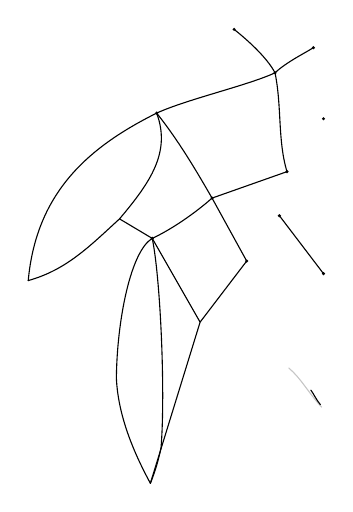
\begin{tikzpicture}[x=.008cm,y=-.008cm,line cap=round,line join=round]
\draw (492,496) .. controls (511,511) and (544,540) .. (557,565)
  .. controls (575,548) and (604,534) .. (618,525);
\draw (557,565) .. controls (514,585) and (417,607) .. (369,629)
  .. controls (263,682) and (178,753) .. (165,895);
\draw (165,895) .. controls (226,878) and (263,840) .. (310,797)
  .. controls (359,739) and (392,691) .. (369,629);
\draw (369,629) .. controls (404,673) and (431,719) .. (457,764)
  -- (576,722) .. controls (561,672) and (568,619) .. (557,565);
\draw (310,797) -- (362,828) .. controls (394,813) and (431,787) .. (457,764)
  -- (512,864) -- (438,961) -- (362,828);
\draw (362,828) .. controls (328,848) and (306,957) .. (305,1050)
  .. controls (308,1116) and (338,1178) .. (359,1217);
\draw (362,828) .. controls (375,891) and (383,1071) .. (376,1160)
  .. controls (371,1185) and (365,1202) .. (359,1217);
\draw (438,961) -- (359,1217);
\draw (564,792) -- (634,884);
% Detached slanting ink stroke beside the graph, not treated as an edge.
\draw[gray!45] (579,1034) .. controls (598,1050) and (610,1073) .. (631,1096);
\draw (614,1069) .. controls (619,1076) and (623,1085) .. (629,1092);
\foreach \x/\y in {492/496,618/525,557/565,369/629,576/722,457/764,362/828,512/864,564/792,634/884,634/638}
  \fill (\x,\y) circle[radius=2.7];
\end{tikzpicture}}
\end{minipage}\hfill
\begin{minipage}[t]{.63\linewidth}
Un graphe est dit \deleted{\unsure{quelq|quelq.|qqch}} \uline{strict} si une arête est connue quand on connait ses sommet.

\deleted{\unsure{Un|On|Une}} La donnée d'un \uline{graphe strict} équivaut donc \unsure{à 2|à la} donnée d'un ens. $S$, et d'une partie $A$ de $\unsure{\mathfrak{P}|\mathcal{P}}_{2}(S)$ (ens des parties de card. 2 de $S$).
\end{minipage}

Arc d'un graphe (ou arête orientée) -- ens $\vec A$

\deleted{\uline{\unsure{Remarque}}} Réalisation topologique d'un graphe
\[
\deleted{X(S,A,R)=\bigl(S\amalg(\vec A\times I)\bigr)/.}
\]

a) Segment associé à un ens $a$ de card. 2
\[
\begin{aligned}
\bigl[\,\deleted{\unsure{\operatorname{réal}|\operatorname{rel}}}\inserted{\operatorname{seg}}(a)&\subset I^{a}\qquad (I=[0,1])\\
\operatorname{seg}(a)&=\bigl\{\{t_{\unsure{n|x}}\}_{n\in a}\mid\textstyle\sum t_n=1\bigr\}\ ;\ \text{on a \unsure{:} }\ a\hookrightarrow\operatorname{seg}(a)
\end{aligned}
\]

b)
\[
\operatorname{réal}(S,A,R)=\left(S\amalg\coprod_{a\in A}\operatorname{seg} R\{a\}\right)\big/\begin{aligned}&\text{\unsure{relation}}\\&\text{d'équiv.}\end{aligned}
\]

\noindent\begin{minipage}[t]{.78\linewidth}
\deleted{Réalisation} \quad [ \unsure{Si|On} a $X=\coprod_{a\in A}\operatorname{seg}R\{a\}$, on a
\end{minipage}\hfill
\begin{minipage}[t]{.20\linewidth}
\diagram{\begin{tikzcd}[ampersand replacement=\&,row sep=0.2em,column sep=1.7em]
\partial X \arrow[r] \& S\\[-2pt]
\cap \& {}\\[-2pt]
X \& {}
\end{tikzcd}}
\end{minipage}
et on ``\unsure{attache}'' $X$ \unsure{:|à} $S$ \unsure{$\vdash$|par} $\partial X\to S$ \quad ]

``Réalisation \inserted{\unsure{géom}} rectiligne'' d'un graphe (fini..) dans un vectoriel (de dim finie\ldots) sur $\mathbb{R}$ : homéom. dans
% archive sheet number: 3

\scanpage{5}
\[
\operatorname{réal}(S,A,R)\lhook\joinrel\longrightarrow E
\]
telle que l'image d'un arc soit un segment.

\uline{Prop} Pour qu'un graphe fini admette une réalisation géom. rectiligne, (dans un vectoriel convenable sur $\mathbb{R}$) il f et s qu'il \deleted{a} soit strict -- et alors il admet une réalisation rectiligne dans $\mathbb{R}^{3}$. De façon précise, si $S\hookrightarrow\deleted{\unsure{\mathbb{R}^{3}|R^{3}}}E$ \inserted{$(\simeq\mathbb{R}^{3},\ \unsure{\text{v. ex.}|\text{p. ex.}|\text{v. a.}})$} est une immersion telle que
% Pencil drawing in the left margin beside the conditions. The small dark marks are reproduced without assigning them vertex status.
\reversemarginpar
\margin{\figure{\begin{tikzpicture}[x=.014cm,y=.014cm,line cap=round,line join=round]
\draw[line width=.65pt] (0,0) ellipse (4.6 and 3.4);
\draw[line width=.8pt] (3,3)--(78,86);
\fill (76,84)--(75,91)--(80,88)--(83,90)--(83,84)--(79,82)--cycle;
\draw[line width=.35pt] (88,98)--(147,158);
\draw[line width=.8pt] (147,155)--(147,162);
\draw[line width=.8pt] (-.4,-9)--(.4,-6);
\end{tikzpicture}}}
\normalmarginpar
\[
\forall x,y\in S\quad x\ne y,\quad\text{on ait}\quad
\deleted{\unsure{\{|\exists}}
\underbrace{\overline{x,y}}_{\substack{\text{segm}\\\text{joignant}\\x\ \text{à}\ y}}\cap S=\{x,y\},
\]
\inserted{(i.e. trois points \inserted{distincts} jamais alignés)}
\inserted{et $\forall x,y,z,t$ distincts, $(\overline{x,y})\cap(\overline{z,t})=\varnothing$}

$\exists 1$ réalis géom. rectiligne $\unsure{\operatorname{réll}|\operatorname{réel}}(S,A,R)\lhook\joinrel-E$ qui $f$ \unsure{pro\(\overset{?}{l}\)onge|prolonge}\ldots

Graphe connexe $=$ réal. géom \unsure{connex|connexe} $=$ qui n'est pas \deleted{\unsure{réunion}} ``somme'' de deux autres graphes $\ne\varnothing$

\uline{NB} Tout graphe est de façon unique réunion de graphes connexes \inserted{et disjoints}

[ graphe somme : $S\amalg S',\quad A\amalg A',\quad R\amalg R'\ \ldots$ ]

% A curved arrow in the left margin starts beside NB and points to Graphe, not to the circled insertion multi.
\reversemarginpar
\margin{\figure{\begin{tikzpicture}[baseline=-.5ex,x=1cm,y=1cm]
\draw[->] (.48,1.1) .. controls (-.18,.95) and (-.35,.25) .. (.05,.18) .. controls (.25,.12) and (.48,.08) .. (.78,0);
\end{tikzpicture}}}
\normalmarginpar
% The heading and bracketed degree condition share a baseline; the two additions stand above them.
\[
\begin{array}{@{}l@{\qquad}l@{}}
&\inserted{\text{(ou \uline{contour} (combinatoire))}}\\[-.3ex]
\text{Graphe }\overset{\text{\inserted{\tikz[baseline=(m.base)]{\node (m) at (0,0) {multi};\draw (0,0) ellipse (.50cm and .20cm);}}}}{\text{polygonal}}
&\bigl[\quad\forall s\in S,\quad\operatorname{card}R\{s\}=2\quad\bigr]
\end{array}
\]

Dualité des \deleted{graphes polygonaux} contours (combinatoires).

\deleted{\unsure{donq|donc}} les composantes \inserted{\unsure{conn|conn.|connexes}} d'un \deleted{graphe polygonal}\inserted{contour} sont \deleted{polygonales.} des contours.

Classification des \deleted{graphes polygonaux}\inserted{contours} conn. $\ne\varnothing$

\uline{Prop} Un \deleted{graphe polyg.}\inserted{contour} connexe \inserted{$\ne\varnothing$} est connu à isom. près quand on connait $\operatorname{card}S$ ($=\operatorname{card}A$), qui est n'importe quel cardinal \deleted{fini ou infini}
\[
2\le c\le\aleph_{0}
\]
(strict \unsure{sss|ssi} $c\ne2$ i.e. $c\geqslant3$)
% archive sheet number: 4

\scanpage{6}
Ils correspondent aux \unsure{sous-groupes|sous-grpes} \inserted{$H$} de $\mathbb{Z}$, distincts de $\mathbb{Z}$ ($c=\operatorname{card}\mathbb{Z}/H$).....

\uline{Orientation d'un contour} : \deleted{\unsure{Ch.|En.}}

\uline{Prop} Soit\deleted{\unsure{s|x}} $X=(S,A,R)$ un contour \inserted{\deleted{\unsure{strict}}} connexe $\ne\varnothing$.

\noindent\begin{minipage}[t]{.28\linewidth}
\figure{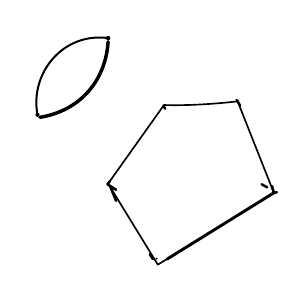
\begin{tikzpicture}[x=.0078cm,y=-.0078cm,line cap=round,line join=round]
\path[use as bounding box] (60,410) rectangle (470,810);
\draw[line width=.72pt] (76,552) .. controls (63,484) and (118,417) .. (191,427);
\draw[line width=1.25pt] (191,433) .. controls (187,495) and (147,545) .. (80,556);
\fill (76,552) circle[radius=3.4];
\fill (191,427) circle[radius=3.7];
\draw[line width=.6pt] (191,664) -- (282,536)
  .. controls (316,537) and (358,535) .. (402,530)
  -- (461,679) -- (272,796) -- cycle;
\draw[line width=1.05pt] (287,787) -- (461,679);
\draw[line width=.9pt] (194,660)--(190,665)--(204,674)
  (195,670)--(204,692)
  (281,537)--(284,542)
  (400,528)--(402,530)--(406,537)
  (458,668)--(461,679)--(466,678)
  (441,665)--(450,670)
  (259,779)--(264,787);
\fill (270,786) circle[radius=1.8];
% The detached strokes and patches are reproduced as ink, not assigned vertex or arrow semantics.
\end{tikzpicture}}
\end{minipage}\hfill
\begin{minipage}[t]{.68\linewidth}
a) \deleted{Un}\inserted{Soit $g$ un} autom. $g$ de $X$ \deleted{est dit \uline{\unsure{direct}}.}\inserted{Conditions équiv.}

\noindent\begin{tabular}{@{}p{.30\linewidth}@{\quad}p{.63\linewidth}@{}}
\unsure{\uuline{d'orientation}|\deleted{\uline{d'orientation}}} & $1^{\circ})$ \deleted{si} $\forall s\in S$, $s$ est lié à $gs$ \\
\deleted{\unsure{$\{$|$f$}} & $2^{\circ})$ $\forall a\in A\quad ga$ est lié à $a$
\end{tabular}


\deleted{\unsure{def.|déf.|b)|Si}} On dit que $g$ est une \deleted{\unsure{autom.} d'}\uline{orientation} de $X$.
\end{minipage}

b) Soit $\omega(X)$\inserted{$\subset\operatorname{Aut}(X)$} l'ens des\unsure{.} \deleted{\unsure{autom.} d'}\unsure{orientation|orientations} de $X$

\inserted{Si $g\in\omega(X)$, on a $g^{-1}\in\omega(X)$.}

Alors $\operatorname{card}\omega(X)=2$ \unsure{;|,} \deleted{et si $g\in\unsure{\omega|\omega(X)}$} \inserted{(si $X$ est strict i.e. si $c=\operatorname{card}S\ne2$)} , et si $g\in\omega(X)$, on a $\omega(X)=\{g,g^{-1}\}$.

c) \deleted{Soit $\operatorname{Aut}^{+}(X)\subset\operatorname{Aut}(X)$ le ss-grpe de $\operatorname{Aut}X$ formé par les $g\in\operatorname{Aut}X$ tels que $g$ opère \unsure{triv$^{\mathrm{lt}}$|triv$^{\mathrm{t}}$} sur $\omega(X)$ [i.e.}

Considérons $\operatorname{Aut}(X)\unsure{-|\to}\operatorname{Aut}(\omega(X))\simeq\mathbb{Z}/2\mathbb{Z}$.

C'est un hom surjectif, i.e. le noyau $\operatorname{Aut}^{+}(X)$ est un ss-grpe d'indice $2$.

De plus, $\operatorname{Aut}^{\unsure{e|\varepsilon|c|+}}(X)$ est un groupe cyclique engendré par tt $g\in\omega(X)$.

\uline{Corollaire} $\operatorname{Aut}(X)\simeq\mathbb{Z}/2\mathbb{Z}\cdot\mathbb{Z}/H$ \inserted{(\unsure{produit|produits} $\frac{1}{2}$ direct):}, où $H$ \unsure{est|$\to$} le ss-grpe de $\mathbb{Z}$ formé des $n\in\mathbb{Z}$ tels que $g^{n}=1$ ($g$ \unsure{etant|etans|dans} une orientation fixé)
% archive sheet number: 5

\scanpage{7}
\uline{connexe} \uline{orienté} ``revient au $=$'' que de se donner un $n\in\mathbb{N}$, $n\geq2$, et un \inserted{tel} torseur sous $\mathbb{Z}/n\mathbb{Z}$ (savoir $S$, \unsure{ou|--} $A$ \unsure{au|--} choix -- NB $\unsure{r|\sigma}:S\longrightarrow A$ est compatible avec l'action de $G^{\unsure{0|\circ}}=\mathbb{Z}/n\mathbb{Z}$ i.e. avec l'action de $u_{\omega}$.

Se donner un \uline{contour connexe} équivaut : la donnée de

$1^{\circ})$ un \unsure{gpe|grpe} cyclique $G^{0}$ (d'ordre $n\geq2$)

$2^{\circ})$ une \deleted{\unsure{ens|un}} partie de $G^{0}$ \deleted{formée d'} de \unsure{la|2} forme $\{g,\unsure{s|g}^{-1}\}$, où $g$ est un générateur \inserted{(\unsure{donc|des} partie de card $2$ \unsure{sss|ss|ssi} $n\ne2$)}

$3^{\circ})$ Un torseur $S$ sous $G^{0}$

$\bullet$ Du moins si $n\geq3$ \deleted{\unsure{sinon|si on}} ; pour une description

$\bullet$ générale, il faut de plus se donner, en lieu du $2^{\circ}$, un

$2$ bis) un ens $\Omega$ à deux \unsure{éléts|élémts|éléments}, et une application $\Omega\xrightarrow{i}G$ telle que, si $\Omega=\{a,b\}$, on ait $i(a)i(b)=1$, $i(a)$ gén. de $G$

% Short rising separator stroke.
\figure{\begin{tikzpicture}[x=1cm,y=1cm]
\draw[line width=.4pt] (0,0) -- (1,.11);
\end{tikzpicture}}

Contour orienté (pas néc. \unsure{connexe|connexe.}) $=$ ensemble sur lequel $\mathbb{Z}$ opère (i.e \unsure{avec|ou} autom \unsure{$u$|$n$})

Contour (pas néc connexe) $=\unsure{\ldots|un}$
% archive sheet number: 6

\scanpage{8}
Orientation d'un contour.

Choix pour \unsure{tte|toute} arête $a\in A$ d'une ``orientation de $a$'' i.e. d'une origine $\deleted{\unsure{\omega|o}}\sigma(a)$ de $a$, de telle façon que l'on ait

\reversemarginpar
% slanted; the separator below and to the right of the note is retained.
\margin{\figure{\begin{tikzpicture}[scale=.43,transform shape]
\node[inner sep=0,anchor=south west] at (0,0) {\begin{minipage}{5.1cm}
\diagram{\begin{tikzcd}[ampersand replacement=\&,column sep=small] A \arrow[r,"{\substack{\sigma\\[-.35ex]\sim}}"] \& S \end{tikzcd}}
$\forall a\in A\quad\deleted{\unsure{\exists1|\exists}}(\sigma(a),a)\in R$\\
\deleted{$\unsure{\forall s\in S|\forall a\in S},\exists1\,a\in A,$}
\end{minipage}};
\draw[line width=.5pt] (0,-.15)--(4.95,-.15) .. controls (5.05,-.15) and (5.1,-.1) .. (5.15,-.05);
\draw[line width=.5pt] (5.35,.15)--(5.35,1.1);
\draw[line width=.5pt] (5.35,1.22)--(5.35,2.25);
\end{tikzpicture}}}

% The condition label is at the left; its last equation wraps onto the next line.
\begingroup\makeatletter\tagsleft@true\makeatother
\[
\begin{aligned}
&\text{Si}\quad \deleted{R\{s\}=\{a,b\},\ \text{alors }\exists}\quad s\in S,\quad \exists1\ a\in R\{s\}\ \text{tel que}\\
&s=\sigma(a).
\end{aligned}\tag*{(\unsure{O|0})}
\]
\endgroup

Réduction au cas connexe

\margin{\figure{
\begin{tikzpicture}[x=.02cm,y=.02cm]
\draw[->,line width=.6pt] (0,0) .. controls (18,-2) and (39,-2) .. (56,-1);
\fill (61,0) circle[radius=1.7];
\draw[->,line width=.65pt] (62,0) .. controls (75,5) and (92,15) .. (108,25);
\end{tikzpicture}}}
\uline{Prop} Si $(S,A,R)$ est un contour connexe, il a exactement \uline{deux} orientations ($\omega$ et $-\omega$).

\margin{\figure{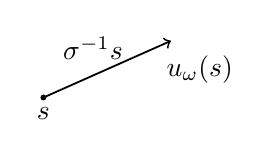
\begin{tikzpicture}[x=.03cm,y=.03cm]
\fill (0,0) circle[radius=1.25];\draw[->,line width=.65pt] (0,0)--(54,24);
\node[below] at (0,0) {$s$};
\node[above] at (21,12) {$\sigma^{-1}s$};
\node[below right] at (48,22) {$u_{\omega}(s)$};
\end{tikzpicture}}}
\deleted{Prop} \uline{Prop} Soit $\omega$ orientation du contour $(S,A,R)$.

$\forall s\in S$, soit $\deleted{\unsure{\omega(s)|w(s)}\unsure{u_{\omega}|u}}\inserted{u_{\omega}}(s)$ l'\uline{extrémité} de l'unique arête \inserted{$\sigma^{-1}(s)$} qui ait \deleted{\unsure{comme}} $s$ comme origine\unsure{.|} $\left[\begin{aligned}(u_{\omega}(s),\sigma^{-1}(s))&\in R,\\u_{\omega}(s)&\ne s\end{aligned}\right]$

\margin{\figure{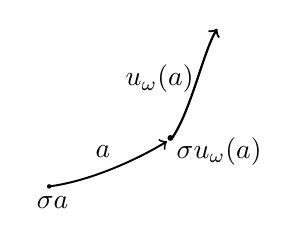
\begin{tikzpicture}[x=.022cm,y=.022cm]
\fill (0,0) circle[radius=1.3];\draw[->,line width=.7pt] (0,0) .. controls (23,3) and (50,15) .. (68,26);
\fill (70,28) circle[radius=1.7];\draw[->,line width=.8pt] (71,28) .. controls (82,44) and (89,78) .. (97,91);
\node[below] at (2,0) {$\sigma a$};\node[above] at (31,11) {$a$};
\node[right] at (68,20) {$\sigma u_{\omega}(a)$};\node[left] at (89,62) {$u_{\omega}(a)$};
\end{tikzpicture}}}
$\forall a\in A$, soit $u_{\omega}(a)$ l'unique arc de $S$ dont l'origine soit l'extrémité de $a$ $\left[\begin{aligned}
(\sigma u_{\omega}(a),a)&\in R,\quad \sigma u_{\omega}(a)\ne\sigma a\\
&\hspace{6em}\text{i.e.}\quad u_{\omega}(a)\ne a
\end{aligned}\right]$

\margin{$\big\}$}Alors $u_{\omega}:(S,\deleted{\unsure{R|B}}A)\unsure{-|\to}(S,A)$ est un autom du graphe $(S,A,R)$. On a $u_{-\omega}=u_{\omega}^{-1}$. Les autom $u_{\omega},u_{\omega}^{-1}$ sont caractérisés par les \deleted{fait que} conditions équivalentes

$1^{\circ})$ $\forall s\in S$, $s$ lié à $gs$

$2^{\circ})$ $\forall a\in A$, $a$ lié à $ga$

Si $n=\operatorname{card}S=\operatorname{card}A$, l'ordre de $u_{\omega},u_{\omega}^{-1}=u_{-\omega}$ est $n$ \unsure{fleche|et} $u_{\omega}\ne u_{-\omega}$ sss $n\ne2$ i.e. $n\geq3$ ; \unsure{donc|alors} $\omega\longmapsto u_{\omega}$ est bijection de $\operatorname{or}(S,A,R)$ \unsure{avec|sur} l'ens des $g\in\operatorname{Aut}(S,A,R)$ satisfaisant les conditions équiv. $1^{\circ}$ \unsure{$-$|ou} $2^{\circ}\unsure{)}\big\}$, Et le \unsure{grpe|gpe} cyclique $\simeq\unsure{Z|\mathbb{Z}}/nZ$ engendré par $u_{\omega}$ est \deleted{formé} \inserted{le} \inserted{\unsure{grpe|gpe} $G^{\unsure{0|\circ}}$} des autom \inserted{orientés} de $(S,A,R,\omega)$ \inserted{\unsure{lire|les|i.e.} de $S,A,R;\omega)$}. $\underset{\unsure{\circ}}{S}$ et $A$ sont des \uline{torseurs} sous $G^{0}$.

\deleted{\unsure{Se|La} donner un}

Torseur sous $\mathbb{Z}/n\mathbb{Z}$ \inserted{$(n\geq1)$} $=$ ensemble \unsure{\deleted{où}à|à} $n$ elément muni d'un ordre \unsure{$^{\times}$|$^{*}$} circulaire. Se donner un contour
\normalmarginpar
% archive sheet number: 7

\scanpage{9}
1) \uline{Ens. avec permutation} $(E,u)\Longleftrightarrow\mathbb{Z}$-ens.

Classification : famille de cardinaux associés aux ss-groupes de $\mathbb{Z}$
\[
=\text{famille de cardinaux}\quad
\begin{tikzpicture}[baseline=-1ex]
\draw[gray!55,line width=.2pt] (0,.08)--(.08,-.10);
\draw[gray!80,line width=.35pt] (.08,-.10)--(.25,.08);
\node[inner sep=0pt] at (.34,.08) {$\unsure{\phantom{x}}$};
\end{tikzpicture}\quad(a_i)_{i\in\mathbb{N}}
\]

\[
E\ \text{fini}\Longleftrightarrow
\underbrace{n_{0}=0}_{\substack{\text{orbites}\\\text{finies}}}
\ \text{et}\quad
\underbrace{\text{les } n_{i}\ \text{finis}}_{\substack{\text{nb fini d'}\\\text{orbites de}\\\text{cardinal } i\in\mathbb{N}\\\text{donné}}},
\quad\underbrace{\text{nuls sauf un nb fini}}_{\text{nb fini d'orbites}}
\]

$u$ transitif ($\Longleftrightarrow u$ définit sur $E$ un ordre circulaire) $\Leftrightarrow$ tous les $n_{i}$ sauf un au plus sont nuls

\uline{Cor} Les classes d'éléments de $\unsure{\mathfrak{S}|\mathscr{S}}_{n}$ mod conjugaison correspondent $1$-$1$\par
\noindent\begin{tabular}{@{}|@{\hspace{.6em}}p{\dimexpr\linewidth-1em\relax}@{}}
aux ``partitions'' de $n$, i.e. aux familles d'entiers $(c_{i})_{1\leq i\leq n}$ tels que
\[
\makebox[\linewidth][l]{$\displaystyle\sum i c_{i}=n$}
\]
\end{tabular}

\diagram{\resizebox{\linewidth}{!}{\begingroup\setlength{\arraycolsep}{2.5pt}\(\begin{array}{ll l|ll l}
\mathfrak{S}_{2}:&2\ \text{\unsure{classes|classe}}&1,\sigma_{12}&\unsure{\mathfrak{A}|\mathscr{A}}_{2}:&1\ \text{classe}&1\\
\mathfrak{S}_{3}:&3\ \text{classes}&1,\sigma_{12},\sigma_{123}&\mathfrak{A}_{3}:&3\ {-}&1,\sigma_{123},\sigma_{321}\\
\mathfrak{S}_{4}:&5\ \text{classes}&1,\sigma_{12},\sigma_{12}\sigma_{34},\sigma_{123},\sigma_{1234}
&\mathfrak{A}_{4}:&\multicolumn{2}{l}{\tikz[baseline=(entry.base)]{
  \node[inner sep=1.5pt] (entry) {$\deleted{\unsure{1|i},\sigma_{\unsure{12|13}}\sigma_{\unsure{34|24}},\sigma_{\unsure{1234|4234}}}$};
  \draw[rounded corners=2.5pt] ([xshift=-2em,yshift=1.5pt]entry.north east)
    -- ([xshift=-2em]entry.north east) -- (entry.north west) -- (entry.south west)
    -- ([xshift=-1.65em]entry.south east) -- ([xshift=-1.65em,yshift=-1.5pt]entry.south east);
}}\\
\mathfrak{S}_{5}:&?&&&&
\end{array}\)\endgroup}}

2) \uline{Rectification} Les contours orientés correspondent aux ens. à permutation $(E,u)$ tels que $u$ n'\uline{ait pas de pt fixe} (car on ne veut pas de polygone à $1$ coté, ds les graphes !)

3) Produit $\frac{1}{2}$ direct de gpes

\diagram{\begin{tikzcd}[ampersand replacement=\&,column sep=small]
\text{donner}\&[-1ex]1 \arrow[r,dash] \& \mathbb{Z}\arrow[r,dash,"i"] \& G\arrow[r,dash,"p"] \& \Gamma\arrow[l,bend left=24,"q"']\arrow[r,dash] \& 1q \&[-1ex] \unsure{p|q}qp=\operatorname{id}_{\Gamma}\quad\unsure{q|p}
\end{tikzcd}}
(suite exacte, avec $q$ un hom. de \unsure{gpes|groupes})

revient à donner
\diagram{\begin{tikzcd}[ampersand replacement=\&,column sep=small,row sep=0pt]
1\arrow[r,dash] \& Z\arrow[r,dash] \& G\arrow[r] \& \Gamma\arrow[r,dash] \& 1 \& p\mid\Gamma'\simeq\deleted{\unsure{\mathrm{iso}|\mathrm{is}}}\Gamma\ \text{\unsure{iso|is}}\\
\& \& \rotatebox{90}{$\subset$} \\
\& \& \Gamma'
\end{tikzcd}}

ou à donner \unsure{grs|gpes} $Z,\Gamma$ avec op. de $\Gamma$ sur $Z$
\[
\Gamma\longrightarrow\operatorname{Aut}_{\mathrm{gr}}(Z)
\]

loi de composition sur $G=\mathbb{Z}\times\Gamma$

% left margin note, slanted; the diagonal divider is retained
\reversemarginpar
\margin{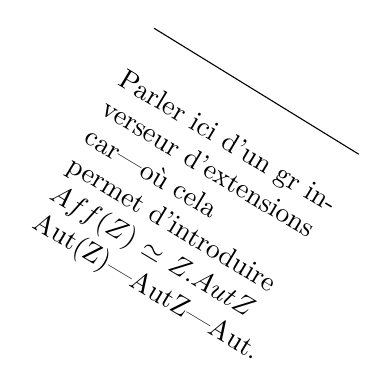
\begin{tikzpicture}
\draw (0,0.4)--(2.6,-1.2);
\node[anchor=north west,rotate=-31,align=left,text width=3.2cm,inner sep=0pt] at (-0.35,-0.1)
{\unsure{Parler} ici d'un gr inverseur d'extensions \unsure{car|où} cela permet d'introduire $\operatorname{Aff}(Z)\simeq Z.\operatorname{Aut}Z$ \deleted{\unsure{Aut(Z)|AutZ|Aut}}.};
\end{tikzpicture}}
\normalmarginpar

\[
\begin{aligned}
&\deleted{(\gamma,z)(\gamma',z')=(\gamma\gamma',\operatorname{int}(\gamma')^{-1}(z).z')}\\
&(z,\gamma)(\unsure{z'|{\mathcal Z}'},\gamma')=(z\operatorname{int}(\gamma)(z'),\gamma\gamma')
\end{aligned}
\]

% Lower-right note with its oblique divider and the short adjacent stroke.
\margin{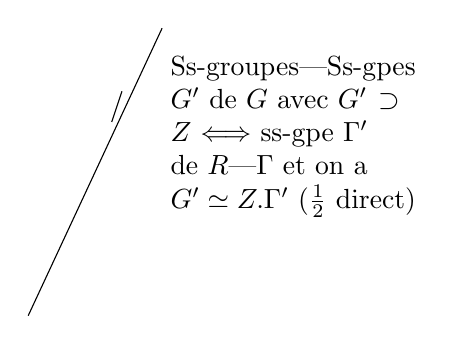
\begin{tikzpicture}
\draw (0,-3.5)--(1.7,0.15);
\draw (1.06,-1.04)--(1.19,-0.65);
\node[anchor=north west,align=left,text width=3.2cm,inner sep=0pt] at (1.8,-0.2)
{\unsure{Ss-groupes|Ss-gpes} $G'$ de $G$ avec $G'\supset Z$ $\Longleftrightarrow$ ss-gpe $\Gamma'$ de \deleted{\unsure{$R$|$\Gamma$}} et on a $G'\simeq\mathbb{Z}.\Gamma'$ ($\frac{1}{2}$ direct)};
\end{tikzpicture}}
% archive sheet number: 8

\scanpage{10}
\uline{Ex}\quad\tikz[remember picture,baseline]\node[inner sep=0pt] (afftitle) {Groupe affine \unsure{associé} à un groupe $\unsure{\mathbb{Z}|Z}$};

\diagram{\begin{tikzcd}[ampersand replacement=\&,column sep=small,row sep=1.2em]
\& \& \operatorname{Aff}(\mathbb{Z})\subset\unsure{\mathfrak{S}|\mathcal{S}}_{\mathbb{Z}_{d}}
   \arrow[d,phantom,"{\rotatebox{18}{$=$}}"{description,xshift=-4.5em}] \& \& \\
1 \arrow[r] \& \mathbb{Z} \arrow[r,"i"] \&
\operatorname{Aut}_{\substack{\text{ens à}\\\text{gr d'op}}}
 (\mathbb{Z},\mathbb{Z}_{d}) \arrow[r,"p"] \arrow[d,hook] \&
\operatorname{Aut}(\mathbb{Z}) \arrow[r] \arrow[l,bend left=29,"q"] \& 1\\
\& \& \operatorname{Aut}(\mathbb{Z})\times\mathfrak{S}_{\mathbb{Z}_{d}} \& \&
\end{tikzcd}}

\noindent\begin{minipage}[t]{.50\linewidth}
\[
\begin{aligned}
&\gamma\in\operatorname{Aut}(\mathbb{Z})\\
&\tikz[remember picture,baseline=(s010qline.base)]{\node[inner sep=0pt] (s010qline) {$q(\gamma)=(\gamma,\gamma)$};}\\
&i(g)=(\mathrm{id}_{\mathbb{Z}},\tau_{g^{\unsure{\prime|.}}}^{\unsure{s|\deleted{s}|\delta}})
  \tikz[remember picture,baseline]\coordinate (idefend);\\
&\boxed{\operatorname{int}(q(\gamma))\mid\mathbb{Z}=\gamma}
\end{aligned}
\]
\end{minipage}\hfill
\begin{minipage}[t]{.45\linewidth}
\diagram{\begin{tikzcd}[ampersand replacement=\&,row sep=.1em]
\underbrace{(\gamma,\rho)\in\operatorname{Aut}(\mathbb{Z},\mathbb{Z}_{d})}\\
\Updownarrow\\
\rho(gx)=\gamma(g)\rho(x)\\
\forall g,x\in\mathbb{Z}
\end{tikzcd}}
\end{minipage}
% Detached upper-gap point and lower i(g) point; only the lower point has uncertain status as writing.
\figure{\begin{tikzpicture}[remember picture,overlay]
\fill ([xshift=5.1em,yshift=.3ex]s010qline.east) circle (.45pt);
\node[inner sep=0pt] at ([xshift=-.15em,yshift=-.65em]idefend) {$\unsure{.}$};
\end{tikzpicture}}

\[
\operatorname{Aff}_{\deleted{\unsure{\substack{\text{ens à}\\\text{gr d'op}}}}}
 (\mathbb{Z})\deleted{\unsure{(\mathbb{Z}_{d})|(G_d)}}\simeq
 \underset{\text{\tikz[baseline=-.4ex]{\draw (0,.04)--(.13,0);}}}{\mathbb{Z}}\mathbin{.}\operatorname{Aut}(\mathbb{Z})
 \qquad\text{\unsure{(produit|produit|(produits|produits} $1/2$ direct)}
\]
% The short oblique stroke below the first product factor is detached; no mathematical role is assigned to it.

Si $\Gamma\subset\operatorname{Aut}(\mathbb{Z})$ ($\Gamma$ ss-groupe) on a un ss-groupe naturel de $\deleted{\unsure{\operatorname{Aut}_{\substack{\text{ens}\\\text{gr d'op}}}(G,G_d)}}\operatorname{Aff}(\mathbb{Z})\deleted{\unsure{=|-}}$, savoir $\operatorname{Aff}^{\Gamma}(\mathbb{Z})\simeq\mathbb{Z}\mathbin{.}\Gamma$.

\noindent\tikz[remember picture,baseline]\coordinate (affblocktop);
Hom d'ens à op. avec \unsure{groupe|groupes} \unsure{variable|variables}
\diagram{\begin{tikzcd}[ampersand replacement=\&,column sep=large]
(E,\unsure{\mathbb{G}|G})\arrow[r,"{(\rho,\gamma)}"']\&(E',\unsure{G'|C'})
\end{tikzcd}}

\deleted{\uline{NB}}

\uline{NB} Si $E'$ est un torseur sous \tikz[baseline=(s010target.base)]{\node[inner sep=0pt] (s010target) {$G'\vphantom{\rule{0pt}{3.8ex}}$};\node[overlay,anchor=base west,inner sep=0pt] (s010nonempty) at ([xshift=.6em,yshift=2.6ex]s010target.base east) {\inserted{et $E\ne\varnothing$}};\draw[overlay] ([xshift=.1em,yshift=-.2ex]s010target.base east) .. controls +(.2em,2ex) and +(1em,0) .. ([xshift=.2em]s010nonempty.south east);}, alors $\rho$ détermine $\gamma$ car \deleted{\unsure{pour}} si $x\in E$, $\forall g\in G$, $\gamma(g)$ est déterminé en termes de $\rho$ par la condition $\rho(g.x)=\gamma(g).\rho(x)$
\tikz[remember picture,baseline]\coordinate (affblockbottom);
\figure{\begin{tikzpicture}[remember picture,overlay]
\draw ([xshift=-.3em]affblocktop.west) .. controls +(-.7em,0) and +(-.25em,.65em) .. ([xshift=-1em,yshift=-.55em]affblocktop.west)
 -- ([xshift=-1em,yshift=.7em]affblocktop.west |- affblockbottom)
 .. controls +(0,-.55em) and +(-.3em,0) .. ([xshift=-.35em]affblocktop.west |- affblockbottom);
\draw[->] ([xshift=-1em,yshift=-.65em]affblocktop.west)
 .. controls +(-3em,2em) and +(-4em,-1em) .. ([xshift=-2em,yshift=-.45em]afftitle.west)
 -- ([yshift=-.45em]afftitle.west) -- ([yshift=.65em]afftitle.west);
\end{tikzpicture}}

Cas $\mathbb{Z}$ \tikz[baseline=(s010vectoriel.base)]{\node[inner sep=0pt] (s010vectoriel) {vectoriel\vphantom{\rule{0pt}{3.8ex}}};\node[overlay,anchor=base west,inner sep=0pt] (s010underlying) at ([xshift=.3em,yshift=2.6ex]s010vectoriel.base west) {\inserted{grpe \unsure{ss-jacent à|s-jacent à|sous-jacent à}}};\draw[overlay] ([xshift=-.2em,yshift=-.2ex]s010vectoriel.base west) .. controls +(-.1em,2ex) and +(1em,0) .. ([xshift=.2em]s010underlying.south east);} $V$ sur corps $R$ (réels p ex)
\[
\begin{aligned}
&\Gamma=\operatorname{Aut}_{R}(V)\subset\operatorname{Aut}_{\mathrm{gr}}(V)\\[.8em]
&\operatorname{Aff}_{R}(V)\simeq V\mathbin{.}\operatorname{Aut}_{R}(V)
\end{aligned}
\]
\[
(\underset{\substack{\rotatebox{90}{$\ni$}\\V}}{z},
 \underset{\substack{\rotatebox{90}{$\ni$}\\\underset{R}{\operatorname{Aut}(V)}}}{\gamma})
 \mathbin{.}(z',\gamma')=(z+\gamma(z'),\gamma\gamma')
\]

Si $V$ muni d'une forme quadratique non \tikz[baseline=(s010deg.base)]{\node[inner sep=0pt] (s010deg) {dég\unsure{,|.}};\node[anchor=south,inner sep=0pt] at ([yshift=1ex]s010deg.north east) {\inserted{$Q$}};} \unsure{on|$\to$} a le groupe des déplacements (transf. affines qui \tikz[remember picture,baseline]\node[inner sep=0pt] (distanceverb) {\unsure{invarient|invariant}}; la distance)
% A separate short stroke stands beneath the opening of the distance verb; its purpose is uncertain.
\figure{\begin{tikzpicture}[remember picture,overlay]
\draw ([xshift=.55em,yshift=-.22em]distanceverb.south west) -- ++(.65em,.02em);
\end{tikzpicture}}
\[
\operatorname{Depl}_{\deleted{\unsure{\text{aff}|\text{Aff}|\text{orth}}}}(V,Q)\simeq V\mathbin{.}\operatorname{Orth}(V,Q)
\]
% archive sheet number: 9

\scanpage{11}
$T$ torseur \unsure{:|à} droite sous \unsure{grp|grpe} $\unsure{\mathbb{Z}|Z}$

\[
\deleted{\unsure{\operatorname{Aut}_{\substack{G\text{-ens}\\G\text{-}\unsure{\mathrm{var}|\mathrm{op}}}}(\unsure{D|T})
 \longrightarrow\operatorname{Aut}(G)}}
\]

\diagram{\begin{tikzcd}[ampersand replacement=\&,column sep=small]
1\arrow[r] \& \mathbb{Z}\arrow[r,"i"] \& \operatorname{Aut}(\mathbb{Z},T)\arrow[r,"p"]
 \& \operatorname{Aut}(\mathbb{Z})\arrow[r,dash]\arrow[l,dashed,bend left=28,"q_t"'] \& 1
\end{tikzcd}}

% A detached short dark mark stands above un; ink versus surface trace is unresolved.
$\forall t\in T$, on a \tikz[baseline=(wordun.base)]{
\node[anchor=base west,inner sep=0pt] (wordun) at (0,0) {un};
\node[inner sep=0pt] at (.30,.42) {\unsure{\tikz[baseline=-.2ex]{\draw[line width=.6pt,line cap=round] (0,0)--(.05,0);}}};}
splitting $q_t$, défini par
\[
\left\{\begin{aligned}&q_t(\gamma)(t)=t\\&p(q_t(\gamma))=\gamma\end{aligned}\right.
\]

Quelle est la relation entre $q_t$ et $q_{t'}$ ?

On \unsure{avait|aurait} $t'=t.g$, et on trouve
\[
q_{t'}=\operatorname{int}(i(g))\circ q_t
 \;:\; \gamma\longrightarrow i(g)\,q_t(\gamma)\,i(g)^{-1}
\]

[ Pour le vérifier, il suffit de voir que
% The brace starts after int, ends below q_t, and has a displaced slanting equals below it.
\[
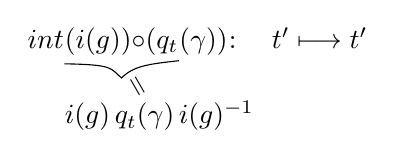
\begin{tikzpicture}[baseline=(proofint.base)]
\node[anchor=base west,inner sep=0pt] (proofint) at (0,0) {$\operatorname{int}$};
\node[anchor=base west,inner sep=0pt] (proofarg) at (proofint.base east) {$(i(g))\unsure{\circ}(q_t$};
\node[anchor=base west,inner sep=0pt] (prooftail) at (proofarg.base east) {$(\gamma))$};
\node[anchor=base west,inner sep=0pt] at (prooftail.base east) {$:\quad t'\longmapsto t'$};
\draw ([yshift=-.10cm]proofarg.south west)
 .. controls +(.65cm,-.01cm) and +(-.15cm,.12cm) .. ([yshift=-.28cm]proofarg.south)
 .. controls +(.15cm,.16cm) and +(-.35cm,-.04cm) .. ([yshift=-.06cm]proofarg.south east);
\node[inner sep=0pt,rotate=-60] at ([xshift=.18cm,yshift=-.40cm]proofarg.south) {$=$};
\node[anchor=north west,inner sep=0pt] at ([yshift=-.57cm]proofarg.south west)
 {$i(g)\,q_t(\gamma)\,i(g)^{-1}$};
\end{tikzpicture}
\]
or \quad $t'=tg$
\[
\begin{aligned}
&\deleted{q_t(\gamma)(t')=q_t(\gamma)(t)\,\gamma(g)=t.\gamma(g)}\\
&\hspace{.3em}\deleted{\operatorname{int}(i(g))\,q_t(\gamma)\,(t')=}\\
&\quad i(g)^{-1}(t')=t\qquad q_t(\gamma)\,i(g)^{-1}(t')=q_{\unsure{b|t}}(\gamma)\,t=t\\
&\qquad i(g)\,q_t(\gamma)\,i(g)^{-1}(t')=tg=t'\qquad\text{ok}\qquad ]
\end{aligned}
\]

\reversemarginpar
\margin{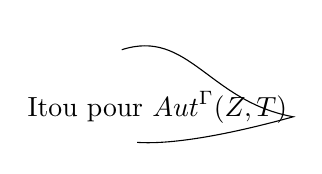
\begin{tikzpicture}[x=.65cm,y=.65cm,baseline=(itou.base)]
\node[anchor=west,inner sep=0pt] (itou) at (0,0) {Itou pour $\operatorname{Aut}^{\Gamma}(\mathbb{Z},T)$};
\draw (1.85,1.13) .. controls (3.15,1.55) and (3.55,.12) .. (5.20,-.18)
 .. controls (4.05,-.50) and (2.88,-.73) .. (2.15,-.68);
\end{tikzpicture}}
\normalmarginpar

% Ex and Z=Z_n are on the baseline of the lower (Aut) row; the canceled fragment lies beneath Z=Z_n.
\[
\begin{aligned}
&\text{\uline{Ex}}\quad \mathbb{Z}=\mathbb{Z}_n\quad
\left\{\begin{aligned}[b]
\operatorname{End}\mathbb{Z}&=\mathbb{Z}_n\\
\operatorname{Aut}\mathbb{Z}&=\mathbb{Z}_n^{*}\supset\{\pm1\}=\Gamma
\end{aligned}\right.\\
&\hspace{3.8em}\deleted{\unsure{\Gamma\in|\Gamma\subset}}
\end{aligned}
\]
\margin{(\uline{NB} \unsure{si} $n=2$, $+1=-1$ dans $\mathbb{Z}_n^{*}$\ldots)}

\[
\begin{aligned}
&\operatorname{Aff}(\mathbb{Z}_n)=\mathbb{Z}_n\mathbin{.}\mathbb{Z}_n^{*}
 \quad\text{(produit ${}^1\! /\! {}_2$ direct)}
 \quad\raisebox{.7em}{\unsure{\tikz[baseline=0pt]{\fill (0,0) circle (.4pt);\fill (.05,.075) circle (.4pt);}}}\\[-.3em]
&\text{\llap{\tikz[baseline=-.1ex]{\draw[line width=.7pt,line cap=round] (0,.04)--(0,0)--(.025,0);}\hspace{1.6em}}}
 \hspace{1.7em}\rotatebox{90}{$\subset$}\\[-.3em]
&\hspace{.5em}\operatorname{Aff}^{\{\pm1\}}(\mathbb{Z}_n)=\mathbb{Z}_n\mathbin{.}\{\pm1\}
\end{aligned}
\]
% The upper-right points have uncertain writing status. The separate lower-left stroke is drawn without assigned function.
\margin{groupe diédral d'indice $n$, $\mathbb{D}_n$ (on suppose $n\ne2$\ldots)}

Soit $T$ torseur sous $Z$ groupe cyclique d'ordre $n\geq3$ muni d'une famille $\{u,u^{-1}\}$ de 2 gén. \tikz[baseline=(old.base)]{
\node[anchor=base west,inner sep=0pt] (old) at (0,0) {\deleted{\unsure{d'ordre $n$}.}};
\node[anchor=south west,inner sep=0pt] at ([yshift=.14em]old.north west)
 {\inserted{inverses l'un de l'}};}autre.
\diagram{\begin{tikzcd}[ampersand replacement=\&,column sep=small]
1\arrow[r] \& Z\arrow[r,dash,"i"] \& \operatorname{Aut}^{\pm1}(T,Z)\arrow[r,dash,"p"]
 \& \{\pm1\}\arrow[r,dash]\arrow[l,bend left=25,"q"{auto=false,inner sep=0pt}] \& 1
\end{tikzcd}}
% archive sheet number: 10

\scanpage{12}
Donnée de $q$ équivaut : \unsure{l|la} donnée de
$\sigma\in
\tikz[baseline=(aut.base)]{
  \node[inner sep=0pt] (aut) {$\operatorname{Aut}^{\pm1}$};
  % Two tiny detached traces above the left of A; writing or surface marks uncertain.
  \node[anchor=south,inner sep=0pt] at ([xshift=-.12em,yshift=.12em]aut.north west)
  {\unsure{\tikz[x=1mm,y=1mm]{\fill (0,.65) circle (.12);\fill[opacity=.45] (0,0) ellipse (.10 and .16);}}};
}(\unsure{G|Z},T)$
\[
\left\{\begin{aligned}p(\sigma)&=-1\\ \sigma^2&=1\end{aligned}\right.
\]
\[
\begin{aligned}
&q_t(-1)=\sigma_t\\[.6ex]
&\sigma_{tg}=g\,\sigma_t\,g^{-1}
=g\,\underbrace{\sigma_t\,g^{-1}\,\sigma_t^{-1}}_{g}\,\sigma_t
=g^2\,\sigma_t=\sigma_t\,g^{-2}\\
&\hspace{15em}\boxed{\sigma_{tg}=g^2\sigma_t=\sigma_t g^{-2}}
\end{aligned}
\]

\uline{Corollaire} Si $n$ impair, $t\longmapsto\deleted{\unsure{q|g}}\sigma_t$ est une bijection de $T$ avec l'ens \deleted{\unsure{des}} $p^{-1}\{-1\}$; donc si on a un \unsure{pl.|pol.} à un nb impair de cotés, l'applic\textsuperscript{n} $t\longmapsto\sigma_t$ qui, à tt sommet du polygone, associe l'unique autom non orienté qui fixe ce sommet, est bijection.

\uline{NB} Si $n$ pair, \unsure{\deleted{elle}|elle} \unsure{ce} n'est pas bijectif, \deleted{\unsure{mais}} \deleted{\unsure{pour tt}} ses fibres sont vides ou de cardinal 2\ldots

% slanted left margin note; the line nodes preserve the cramped oblique geometry.
\reversemarginpar
\margin{\vspace*{-2.7\baselineskip}\hspace*{-1.05cm}%
\begin{tikzpicture}[x=.007cm,y=.007cm,baseline=(0,0)]
  \node[anchor=base west,rotate=34,inner sep=0pt] at (31,-115) {$\{u,\bar u\}\subset Z$};
  \node[anchor=base west,rotate=34,inner sep=0pt] at (15,-183) {gén. opposés d'ordre};
  \node[anchor=base west,rotate=34,inner sep=0pt] at (10,-239) {$n=2m$, alors};
  \node[anchor=base west,rotate=34,inner sep=0pt] at (30,-291) {$u^m=\bar u^m=s$, \uline{unique}};
  \node[anchor=base west,rotate=34,inner sep=0pt] at (23,-348) {\uline{\unsure{élémt|élément} d'ordre} 2 de $Z$};
  \node[anchor=base west,rotate=34,inner sep=0pt] at (25,-412) {appelé \unsure{symétrie|symetrie}};
  \node[anchor=base west,rotate=34,inner sep=0pt] at (25,-465) {Mon $\sigma_t=\sigma_{t'}$};
  \node[anchor=base west,rotate=34,inner sep=0pt] at (35,-520) {\unsure{sss|ssi} $t,t'$ sont \unsure{conjugués}};
  \node[anchor=base west,rotate=34,inner sep=0pt] at (43,-565) {mod $\{1,s\}$};
  % The separate upright and the thinner curved boundary are not mathematical arrows.
  \draw[line width=.45pt] (313,-5) -- (319,-179);
  \draw[line width=.28pt] (285,-73) -- (307,-154)
    .. controls (337,-187) and (393,-193) .. (427,-193)
    .. controls (377,-221) and (337,-255) .. (335,-281)
    .. controls (342,-359) and (375,-401) .. (334,-476)
    .. controls (291,-536) and (222,-603) .. (152,-665);
\end{tikzpicture}}
\normalmarginpar

\uline{Sommet} \uline{opposé}, symétrie canonique

\uline{Parenthèse}\qquad Produit fibré d'ens

\diagram{\begin{tikzpicture}
\node[anchor=north west,inner sep=0pt] (square) at (0,0) {\begin{tikzcd}[ampersand replacement=\&,column sep=2em,row sep=2.4em]
E\arrow[r,"p"] \& \unsure{S|B}\\
P\arrow[u,dashed,"q'"]\arrow[r,dashed,"p'"] \& F\arrow[u,"q"']
\end{tikzcd}};
% The set description begins at the level of the lower row of the square.
\node[anchor=north west,inner sep=0pt] at (4.5,-1.5) {$\begin{aligned}
&P\subset E\times F\\[-.4em]
&\hspace{.3em}\rotatebox{90}{$=$}\\[-.4em]
&\{(x,y)\mid px=qy\}
\end{aligned}$};
\end{tikzpicture}}

% Detached pair of points to the far right of the set display; no punctuation function assigned.
\margin{\raisebox{1.2em}{\unsure{\tikz[x=1mm,y=1mm]{\fill (.45,.8) circle (.12);\fill (0,0) circle (.12);}}}}

% Detached, definite ink stroke above Solution; no lexical value is assigned.
\figure{\makebox[\linewidth][l]{
\begin{tikzpicture}[x=1cm,y=1cm]
\fill (0.025,0.29) .. controls (-0.015,0.28) and (-0.012,0.19) .. (0.018,0.15)
 .. controls (0.038,0.12) and (0.039,0.075) .. (0.012,0.055)
 .. controls (-0.005,0.039) and (-0.036,0.055) .. (-0.043,0.037)
 .. controls (-0.044,0.008) and (0.003,-0.004) .. (0.028,0.022)
 .. controls (0.071,0.06) and (0.06,0.12) .. (0.05,0.17)
 .. controls (0.072,0.23) and (0.062,0.27) .. (0.025,0.29) -- cycle;
\end{tikzpicture}}}

Solution d'un Pb universel dans la cat. des ens :

Si $E,F,S$ des \unsure{grpes|groupes}, $p,q$ hom de \unsure{grpe|groupe}, alors $P$ un \unsure{grpe|groupe} (et solution du pb univ. analogue \unsure{ds|dans} cat. des \unsure{grpes|groupes})
\[
\operatorname{Ker}p\sim\operatorname{Ker}p',\quad
\operatorname{Ker}q\sim\operatorname{Ker}q'
\]

Si $p$\tikz[baseline=(surj.base)]{
  \node[anchor=base west,inner sep=0pt] (surj) at (0,0) {surjectif};
  \node[anchor=base west,inner sep=0pt] at (-.05, .39) {\inserted{$:E\mathbin{\text{---}}S$}};
  \draw[line width=.3pt] (.02,.12) .. controls (.24,.32) and (.65,.30) .. (.94,.40);
}\ bijectif) alors $P\mathbin{\text{---}}F$ surjectif bijectif).

[Langage des
\tikz[baseline=(old.base)]{
  \node[anchor=base,inner sep=0pt] (old) at (0,0) {\deleted{\unsure{diagrammes}}};
  \node[anchor=base,inner sep=0pt] at (.12,.38) {\inserted{carrés}};
}
cartésiens]

Image inverse d'ex. de \unsure{grpe|groupe|grpes|groupes}
% archive sheet number: 11

\scanpage{13}

\diagram{\begin{tikzcd}[ampersand replacement=\&,column sep=2em,row sep=2.2em]
1\arrow[r]\&Z\arrow[r,phantom,"\unsure{-|\to}" description]\&G\arrow[r,dash]\&\Gamma\arrow[r,dash]\&1\&[3em](E)\\
1\arrow[r,phantom,"\unsure{-|\to}" description]\&Z\arrow[u,"\unsure{2|\wr}"']\arrow[r,dash]\&G'\arrow[u]\arrow[r,dash]\&\Gamma'\arrow[u]\arrow[r,dash]\&1\&(E')
\end{tikzcd}}

Si l'extension $(E)$ \unsure{splitte|splitt.}, l'ext. $E'$ aussi.

\noindent
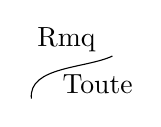
\begin{tikzpicture}[baseline=(t.base)]
  \node[anchor=base west,inner sep=0pt] (t) at (0,0) {Toute};
  \node[anchor=base west,inner sep=0pt] at (-.32,.60) {\inserted{Rmq}};
  \draw (.64,.48) .. controls (.30,.32) and (-.43,.35) .. (-.39,-.06);
\end{tikzpicture}
extension splittée $G$ de un $\Gamma$ par un $Z$ provient par image inverse d'\deleted{\unsure{une}}l'ext. splittée
\[
\begin{tikzpicture}[baseline=(za.base)]
  \path[use as bounding box] (0,-.1) rectangle (12,.65);
  \node[anchor=base west,inner sep=0pt] (za) at (0,0) {$Z.\operatorname{Aut}(Z).$};
  % Detached two-lobed trace; writing versus surface trace remains uncertain.
  \node[inner sep=0pt] at (8.15,.40) {\unsure{\begin{tikzpicture}[baseline=0pt]
    \fill (-.006,.048) ellipse[x radius=.018cm,y radius=.032cm,rotate=24];
    \fill (.002,-.012) ellipse[x radius=.019cm,y radius=.037cm,rotate=12];
  \end{tikzpicture}}};
\end{tikzpicture}
\]

\figure{\begin{tikzpicture}
  \path[use as bounding box] (0,-.06) rectangle (12,.55);
  \draw (4.75,.28)--(7.12,.38);
  \draw (4.83,.08)--(6.96,.10);
  % Tiny detached point beneath the lower rule endpoint; possible surface trace.
  \node[inner sep=0pt] at (6.98,.015) {\unsure{\begin{tikzpicture}[baseline=0pt]
    \fill (0,0) ellipse[x radius=.009cm,y radius=.011cm];
  \end{tikzpicture}}};
  % Isolated point to the right of the divider; possible surface trace.
  \node[inner sep=0pt] at (10.02,.13) {\unsure{\begin{tikzpicture}[baseline=0pt]
    \fill (0,0) ellipse[x radius=.024cm,y radius=.021cm,rotate=-16];
  \end{tikzpicture}}};
\end{tikzpicture}}

4) \quad Ens. de petit cardinal

a) \uline{Cardinal 2}\qquad Ens de cardinal 2 $\longleftrightarrow$ \unsure{torseur|torseurs} \unsure{sur|sous} $\mathbb{Z}_2$ ou encore, \uline{espace affine \unsure{\deleted{sous}|\deleted{sur}|sous|sur}} $\deleted{\unsure{\mathbb{Z}|Z}}\mathbb{F}_2$ (ou encore, \deleted{\illegible{1}} espace affine de dim 1 sur corps $\mathbb{F}_2$ --- car les espaces vect. de dim 1 sur $\mathbb{F}_2$ sont can. isomorphes \ldots)

\[
\begin{aligned}
&\begin{tikzpicture}[baseline=(bx.base)]
  \path[use as bounding box] (-.1,-.08) rectangle (11.3,1.45);
  \node[anchor=base west,inner sep=0pt] (bx) at (.35,.52)
    {$\operatorname{Aff}(1,\mathbb{F}_2)\simeq\operatorname{Aff}(\mathbb{Z}_2)\simeq\unsure{\mathfrak{S}|\mathcal{S}}_2$};
  % The drawn frame has gaps at the upper left and lower right.
  \draw (-.05,1.13)--(8.25,1.43)--(8.36,.43);
  \draw (0,.94)--(.09,0)--(8.30,.24);
  % Detached pair to the right of the box; possible surface trace.
  \node[inner sep=0pt] at (10.94,.67) {\unsure{\begin{tikzpicture}[baseline=0pt]
    \fill (.032,.032) ellipse[x radius=.020cm,y radius=.024cm,rotate=-22];
    \fill (-.020,-.038) ellipse[x radius=.024cm,y radius=.019cm,rotate=12];
  \end{tikzpicture}}};
\end{tikzpicture}\\[-.1em]
&\hspace{4.1cm}(\unsure{\mathcal{A}|A}_2=\{1\})
\end{aligned}
\]

b) \uline{Cardinal 3}
\[
\begin{aligned}
&\mathfrak{S}_3\simeq
\begin{gathered}[t]
  \operatorname{Aff}(1,\mathbb{F}_3)\\[-.15em]
  \rotatebox{90}{$\simeq$}\\[-.15em]
  \begin{aligned}
    \mathbb{F}_3^{+}&\mathbin{.}\mathbb{F}_3^{*}\\[-.4em]
    \rotatebox{90}{$\unsure{\simeq|=}$}&\quad\rotatebox{90}{$=$}\\[-.25em]
    \mathbb{Z}_3&\quad\mathbb{Z}_2
  \end{aligned}
\end{gathered}
\simeq\operatorname{Gl}(2,\mathbb{F}_2)\simeq
\begin{gathered}[t]
  \operatorname{GP}(1,\mathbb{F}_2)\\[-.15em]
  \rotatebox{90}{$=$}\\[-.15em]
  \begin{tikzpicture}[baseline=(qq.base)]
    \node[inner sep=0pt] (qq) at (0,0) {$\operatorname{Gl}(2,\mathbb{F}_2)/\mathbb{F}_2^{*}$};
    % Detached point below the quotient's left portion; possible surface trace.
    \node[inner sep=0pt] at (-1.25,-.58) {\unsure{\begin{tikzpicture}[baseline=0pt]
      \fill (0,0) ellipse[x radius=.010cm,y radius=.013cm];
    \end{tikzpicture}}};
  \end{tikzpicture}
\end{gathered}\\[.55em]
&\hspace{.3cm}\mathcal{A}_3\simeq\deleted{\mathbb{Z}}\mathbb{F}_3^{+}(\simeq\mathbb{Z}_3)
\end{aligned}
\]
% archive sheet number: 12

\scanpage{14}
c)
\[
\begin{aligned}
\unsure{\mathfrak{S}|\mathcal{S}}_4&\simeq\operatorname{Aff}\,2,\mathbb{F}_2)\simeq\operatorname{GP}(1,\mathbb{F}_3)\\
\unsure{\mathfrak{A}|\mathcal{A}}_4&\simeq\operatorname{Aff}(1,\mathbb{F}_4)\qquad ?
\end{aligned}
\]

% Two detached points at the right of c), between its two formula baselines;
% writing versus surface trace remains uncertain, with no punctuation assigned.
\margin{\figure{\unsure{\begin{tikzpicture}[x=1mm,y=1mm]
\fill (0,1.2) ellipse [x radius=.15,y radius=.19];
\fill[gray] (-.04,0) ellipse [x radius=.13,y radius=.22];
\end{tikzpicture}}}}

d)
\[
\begin{aligned}
\mathfrak{S}_5&\simeq\operatorname{GP}(1,\mathbb{F}_5)\\
\mathfrak{A}_5&\simeq\operatorname{GP}(1,\mathbb{F}_4)
\end{aligned}
\]

Quelques groupes classiques sur un corps $k$

\diagram{\(\left.
\begin{tikzcd}[ampersand replacement=\&,column sep=small,row sep=1em]
1\arrow[r] \& k^*\arrow[r] \& \operatorname{Gl}(V)\arrow[r] \&\operatorname{GP}(V)\arrow[r,dash]\&1\\
1\arrow[r] \& k^*\arrow[r,dash] \&\operatorname{Gl}(n,k)\arrow[r] \&\operatorname{GP}(n-1,k)\arrow[r]\&1
\end{tikzcd}
\right\}\;\text{ne \unsure{splitte} pas en général}\)}

% slanted, in the left margin; the surrounding line has small gaps at the left.
\reversemarginpar
\margin{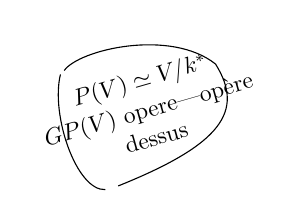
\begin{tikzpicture}[baseline=(proj.base),rotate=16,scale=.85]
\node[inner sep=2pt,transform shape] (proj) {\shortstack{$\mathbb{P}(V)\simeq V/k^*$\\$\operatorname{GP}(V)$ \unsure{opere|opère}\\dessus}};
\draw (-1.05,.88) .. controls (-.75,1.12) and (.65,1.05) .. (1.15,.35)
  .. controls (1.38,-.45) and (.9,-.83) .. (-.75,-1.0);
\draw (-1.12,.84) .. controls (-1.43,.3) and (-1.37,-.9) .. (-.95,-1.0);
\end{tikzpicture}}
\normalmarginpar

\[
\begin{aligned}
\text{Structure de $k$-vectoriel }\tikz[baseline=(vectbase.base)]{
  \node[inner sep=0pt] (vectbase) {sur ens};
  \node[anchor=south west,inner sep=0pt] at ([xshift=-.3em,yshift=.8em]vectbase.north west) {\inserted{de dim $n$}};
  \draw ([xshift=-.35em,yshift=-.4em]vectbase.west)
    .. controls ([xshift=-.7em,yshift=1.0em]vectbase.west) and ([xshift=.4em,yshift=1.1em]vectbase.north west)
    .. ([xshift=.35em,yshift=1.1em]vectbase.north east)
    .. controls ([xshift=.6em,yshift=1.15em]vectbase.north east) and ([xshift=.6em,yshift=1.35em]vectbase.north east)
    .. ([xshift=.4em,yshift=1.35em]vectbase.north east);
}V
&\longleftrightarrow\ \text{donnée d'\unsure{un|une} \unsure{élemt|élémt|élement|élément}}\\
&\qquad\text{de }\operatorname{Isom}_{\text{ens}}(k^n,V)/\operatorname{Gl}(n,k)
\end{aligned}
\]

Structure de $k$-espace affine de dim $n$ sur \deleted{$E$} ens $E$
\[
\begin{aligned}
\longleftrightarrow\ &\text{donnée d'un \unsure{élémt|élément} de}\\
&\operatorname{Isom}_{\text{ens}}(k^n,V)/\unsure{\operatorname{Aff}n,k)|\operatorname{Aff}(n,k)}
\end{aligned}
\]

[ De façon \unsure{général|générale}, \deleted{si $Z$ est un \unsure{groupe|grpe}}, la notion de
\tikz[baseline=(oldaff.base)]{
  \node[inner sep=0pt] (oldaff) {\deleted{espace \unsure{affine|aff.}}};
  \node[anchor=south west,inner sep=0pt] at ([xshift=.8em,yshift=.7em]oldaff.north west)
    {\inserted{torseur (à droite, disons) $E$}};
}
sous \unsure{grpe|groupe} non précisé peut être considéré comme structure sur le seul ens de base $E$,
\tikz[baseline=(oldapp.base)]{
  \node[inner sep=0pt] (oldapp) {\deleted{\unsure{savoir application} $E\times E\times E\,\unsure{\mathbin{\text{---}}|\longrightarrow}\,E$}};
  \node[anchor=south west,inner sep=0pt] at ([xshift=.7em,yshift=.7em]oldapp.north west)
    {\inserted{p.ex. donnée d'un}};
}
\deleted{$(x,y,z)\,\unsure{\mathrel{\mapstochar\relbar\joinrel\relbar}|\longmapsto}\,\unsure{6x|sx|\delta x}$}
couple $\Gamma\subset\mathfrak{S}_{E}$ ss-grpe, tel que \ldots ] ; \unsure{valable} pour ens. à grpe d'op \uline{fidèle}\ldots ]

Une structure d'\uline{espace affine sous} $k$ est alors la donnée d'un tel $\Gamma$, avec \deleted{\unsure{$\Gamma$ com}} comm, \unsure{\deleted{et}|et} un hom d'anneaux unit.
\[
 k\longrightarrow\operatorname{End}_{\mathbb{Z}}(\Gamma)\quad\ldots\qquad ]
\]

Structure de $k$-espace projectif de dim $n$ sur $\unsure{P|\mathbb P}$
\[
\begin{tikzpicture}[baseline=(projective.base)]
\node[anchor=base west,inner sep=0pt] (projective) at (0,0)
 {$\displaystyle\longleftrightarrow\quad\text{donnée de}\quad
 \operatorname{Isom}_{\text{\unsure{ens|ens,}}}\left(
 \underset{\substack{\rotatebox{90}{$=$}\\(k^n-\unsure{(0)|(0}/k^*}}{\mathbb{P}^{n-1}(k)},P\right)
 /\operatorname{GP}(n-1,k)$};
% The enclosure over the arrow is open at its top, not a closed box.
\node[inner sep=0pt,font=\small] at (.35,.70) {déf};
\draw (.02,.87) -- (.02,.45) -- (.68,.45) .. controls (.75,.45) and (.75,.64) .. (.75,.86);
\draw[->] (.36,.45) -- (.36,.12);
% Divider bends below the small quotient and continues rightward.
\draw (2.70,-.77) -- (6.00,-.77)
 .. controls (6.35,-.77) and (6.25,-1.17) .. (6.70,-1.17) -- (11.60,-1.17);
\end{tikzpicture}
\]

\diagram{\begin{tikzcd}[ampersand replacement=\&,column sep=small,row sep=.6em]
\operatorname{Gl}(n,k)\arrow[r]\&\operatorname{Aff}(n,k)\arrow[r]\&\operatorname{GP}(n,k)\\
\substack{\text{vect. de dim $n$}\\\text{sur $k$}}\arrow[r,maps to,"\substack{\text{oubli}\\\text{origine}}"']
\&\substack{\text{espace affine de}\\\text{dim $n$ sur $k$}}
\arrow[r,maps to,"\substack{\text{espace proj.}\\\text{associé à}\\\text{l'esp. vect. \unsure{enveloppant|enveloppe}}}"']
\&\substack{\text{espace projectif}\\\text{de dim $n$ sur $k$}}
\end{tikzcd}}
% archive sheet number: 13

\scanpage{15}
\uline{Exercice}\qquad Réalisation régulière d'un polygône.

Soit $\deleted{V}E$ plan affine euclidien sur $\mathbb{R}$ (avec metrique déf pos. sur \unsure{l'espace|l'esp|l'esp.} $V$ des translations). Une réalisation rectiligne d'un polygone $(S,A,R)$ est dite \uline{régulière} si tous les cotes du polygône ont $=$
% The two-line addition stands to the right of longueur. Its enclosing line is
% open at the left-hand tail; the separate comma remains beside that opening.
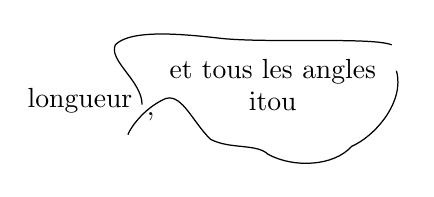
\begin{tikzpicture}[baseline=(longueur.base),x=1cm,y=1cm]
  \node[anchor=base west,inner sep=0pt] (longueur) at (0,0) {longueur};
  \node[anchor=base,inner sep=0pt] at (1.57,-.10) {,};
  \node[anchor=center,inner sep=0pt] at (3.12,.29)
    {\inserted{\shortstack{et tous les angles\\itou}}};
  \draw[line width=.45pt]
    (1.46,.04) .. controls (1.46,.34) and (1.03,.60) .. (1.12,.80)
    .. controls (1.32,1.01) and (2.04,.93) .. (2.48,.88)
    .. controls (3.12,.82) and (4.38,.90) .. (4.63,.80);
  \draw[line width=.45pt]
    (4.69,.47) .. controls (4.80,.08) and (4.42,-.36) .. (4.12,-.49)
    .. controls (3.90,-.74) and (3.39,-.77) .. (3.06,-.59)
    .. controls (2.91,-.45) and (2.58,-.53) .. (2.33,-.40)
    .. controls (2.09,-.17) and (1.95,.23) .. (1.72,.10)
    .. controls (1.48,-.02) and (1.32,-.24) .. (1.28,-.34);
\end{tikzpicture}
\uline{régulière} \deleted{et} \uline{\unsure{normalisee|normalisée}} si la dite longueur est $1$.

a) Existence, grâce à équation cyclotomique $z^n=1$ dans $\mathbb{C}$.

b) Prouver que si $(V\deleted{\unsure{,}}\supset P\deleted{\unsure{,}}\supset\deleted{\unsure{A|B}}S)$ et $(V'\supset P'\supset S')$ sont deux $n$-polygônes ($n\geq3$) munis d'une \unsure{rèal.|réal.} rectiligne \uline{rég.} (resp \unsure{normalisee|normalisée}) il existe une \deleted{\unsure{iso|isom}} similitude (resp \unsure{isom}) \deleted{\uline{unique}} de $V$ sur $V'$, qui transforme $P$ et $P^{\unsure{\prime|!}}$, $S$ en $S'$; \tikz[baseline=(cancel.base),x=1em,y=1em]{
  \node[inner sep=0pt,anchor=base west] (cancel) at (0,0) {\deleted{si $V\unsure{;|,}P,S$}};
  % The cancellation has a separate hooked return at its left end.
  \draw[line width=.4pt] (-.55,.25) .. controls (-.35,-.02) and (.12,-.06) .. (.62,.3);
  \draw[line width=.4pt] (-.55,.25) -- (-.12,.35);
} plus précisément, pour tt isom (comb) de $(\deleted{P}\unsure{S},A,R)$ sur $(S',A',R')$, $\exists\,\unsure{\vert|1}$ similitude
% The addition is above de V. A rising curved arrow runs beneath it and ends
% just above the corrected V; the baseline text remains de V sur V'.
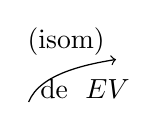
\begin{tikzpicture}[baseline=(de.base),x=1cm,y=1cm]
  \node[anchor=base west,inner sep=0pt] (de) at (.16,0) {de};
  \node[anchor=base,inner sep=0pt] (oldV) at (1.02,0) {$\deleted{\unsure{E}}V$};
  \node[anchor=base west,inner sep=0pt] at (0,.63) {\inserted{(isom)}};
  \draw[->,line width=.45pt] (.02,-.05)
    .. controls (.16,.31) and (.76,.43) .. (1.13,.49);
\end{tikzpicture}
sur $V'$ qui l'induise. \deleted{Montrer que}

\deleted{\unsure{Ex|Cor}}\quad\uline{Cor} Notion d'enveloppe affine (ou vectorielle, grâce : centre de
% The addition is above gravité), with its independent closing parenthesis.
% The curved lead meets short forked strokes and a longer oblique stroke.
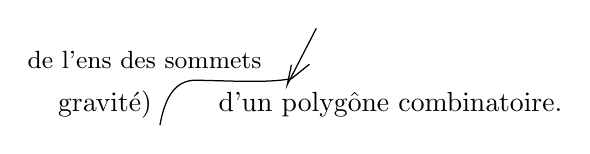
\begin{tikzpicture}[baseline=(gravite.base),x=1em,y=1em]
  \node[anchor=base west,inner sep=0pt] (gravite) at (0,0) {gravité)};
  \node[anchor=base west,inner sep=0pt,font=\small] at (-1.1,1.55)
    {\inserted{de l'ens des sommets}};
  \node[anchor=base west,inner sep=0pt] at (5.8,0) {d'un polygône combinatoire.};
  \draw[line width=.45pt] (3.7,-.5)
    .. controls (3.95,.9) and (4.5,1.18) .. (5.2,1.12)
    .. controls (6.3,1.1) and (7.6,1.02) .. (8.45,1.18);
  \draw[line width=.45pt] (8.45,1.18) -- (9.1,1.70);
  \draw[line width=.45pt] (9.35,3.0) -- (8.30,.96) -- (8.45,1.68);
\end{tikzpicture}

\deleted{\unsure{Si|Soit}} Orientation du polygône $\longleftrightarrow$ orientation de son enveloppe
% Two detached dark points below the right end of the last line: writing versus surface trace remains uncertain.
\par\vspace{2.5\baselineskip}\noindent\hfill
\unsure{\tikz[baseline=-.3ex]{
  \fill (0,0) ellipse (.055em and .035em);
  \fill (.14em,.24em) ellipse (.035em and .055em);
}}\hspace*{2em}\par
% archive sheet number: 14
